\documentclass[tikz,border=2pt]{standalone}
\usepackage{amsmath,amssymb}
\usepackage{tikz}
\usetikzlibrary{matrix}

\begin{document}
% The Cayley table of the group (Z_4, +): every row and column is a permutation of the
% elements, 0 is the identity, and each element has an inverse (where the 0s sit).
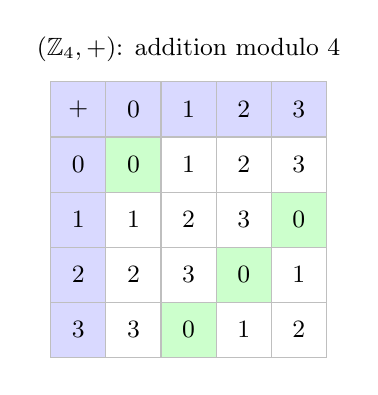
\begin{tikzpicture}[every node/.style={font=\small}]
	\matrix (C) [matrix of math nodes, nodes={minimum size=7mm, anchor=center, draw=gray!50}, column sep=-\pgflinewidth, row sep=-\pgflinewidth] at (0,0) {
		|[fill=blue!15]| + & |[fill=blue!15]| 0 & |[fill=blue!15]| 1 & |[fill=blue!15]| 2 & |[fill=blue!15]| 3 \\
		|[fill=blue!15]| 0 & |[fill=green!20]| 0 & 1 & 2 & 3 \\
		|[fill=blue!15]| 1 & 1 & 2 & 3 & |[fill=green!20]| 0 \\
		|[fill=blue!15]| 2 & 2 & 3 & |[fill=green!20]| 0 & 1 \\
		|[fill=blue!15]| 3 & 3 & |[fill=green!20]| 0 & 1 & 2 \\
	};
	\node[anchor=south] at (C.north) {$(\mathbb{Z}_4,+)$: addition modulo $4$};
\end{tikzpicture}
\end{document}
